\documentclass[11pt, spanish]{report}
\usepackage[spanish]{babel}
\usepackage[utf8]{inputenc}
\usepackage{geometry}
\usepackage{graphicx}
\usepackage{subfig}
\usepackage{caption}
\usepackage{subcaption}
 \geometry{
 a4paper,
 total={170mm,257mm},
 left=20mm,
 top=20mm,
 }
\usepackage{graphicx}
\graphicspath{ {images/} }
\usepackage[utf8]{inputenc}
\decimalpoint

\title{Actividad9}
\author{César Andrés Pérez Robinson }
\date{Mayo 2019}

\begin{document}

\maketitle

\section{Introducción}
En esta actividad, se describe un sistema de dos masas y tres resortes presentadas por Richard Fitzpatrick como se muestra en la Figura 1, y se resuelve utilizando la función odeint de SciPy.
\\ Considerando un sistema mecánico que representa a dos masas idénticas que se unen entre ellas y a dos paredes, libres de moverse en una superficie sin fricción con una constante de los resortes \textit{k}, la posición instantánea del sistema estará especificado por los desplazamientos de las masas $x_1(t)$ y $x_2(t)$. Teniendo las extensiones de los resortes como $x_1$, $x_2-x_1$ y $-x_2$, respectivamente, y asumiendo que $x_1=x_2=0$ corresponde a la configuración del equilibrio, las ecuaciones de movimiento están dadas por:
\begin{figure}[ht]
\caption{Sistema de resortes}
\centering
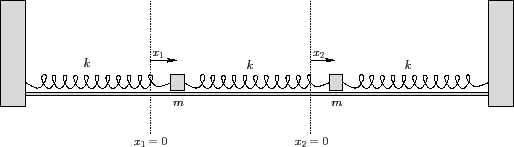
\includegraphics[width=0.65\textwidth]{figura1.png}
\end{figure}
\begin{equation}
    mx''_1=-kx_1+k(x_2-x_1)
\end{equation}
\begin{equation}
    mx''_2=-k(x_2-x_1)+k(-x_2)
\end{equation}
\subsection{Explicación del Cookbook de SciPy}
Con Cookbook de SciPy se puede encontrar la solución numérica del sistema de ecuaciones diferenciales presentado en este problema. \\
El código que presentan para un sistema de dos masas es diferente al de Fitzpatrick, ya que solamente se encuentra una pared al lado izquierdo del sistema de dos masas y dos resortes, por lo que el código debe de ser modificado para nuestra conveniencia. \\
Existe otra diferencia en el código de Cookbook; el sistema de referencia que usan para las longitudes de los resortes comienza de la pared hacia la derecha, mientras que en Fitzpatrick se toma de una posición de equilibrio de cada masa.
\\
Tenemos que para el código de Cookbook, las ecuaciones de su sistema están dadas por
\begin{equation}
    m_1x''_1+b_1x'_1+k_1(x_1-L_1)-k_2(x_2-x_1-L_2)=0
\end{equation}
\begin{equation}
    m_2x''_2+b_2x'_2+k_2(x_2-x_1-L_2)=0
\end{equation}
Tomando que $$x_1=L_1$$ $$x_2-x_1=L_2$$ $$-x_2=L_3$$
podemos reescribir las ecuaciones diferenciales (3) y (4) de tal manera que:
\begin{equation}
    m_1x''_x=-b_1x'_1+k_1(x_1-L_1)-k_2(x_1-L_1+L_2-x_2)
\end{equation}
\begin{equation}
    m_2x''_2=-b_2x'_2-k_3(x_2-L_2)-k_2(x_2-L_2+L_1-x_1)
\end{equation}
También tenemos que
\begin{equation}
    y_1=x'_1
\end{equation}
\begin{equation}
    y_2=x'_2
\end{equation}
Lo que utilizamos para introducir el sistema de cuatro ecuaciones a la función odeint, donde genera un archivo de datos que después podemos graficar para obtener la imagen.
\subsection{Parámetros}
Se tomó que todas las constantes de los resortes fueron igual a uno, el peso de las masas fue igual a uno, las longitudes y las posiciones iniciales fueron iguales. \\
Generando la gráfica se obtiene la Figura 2.
\begin{figure}[ht]
\caption{Grafica de posicion de las masas en el sistema de resortes}
\centering
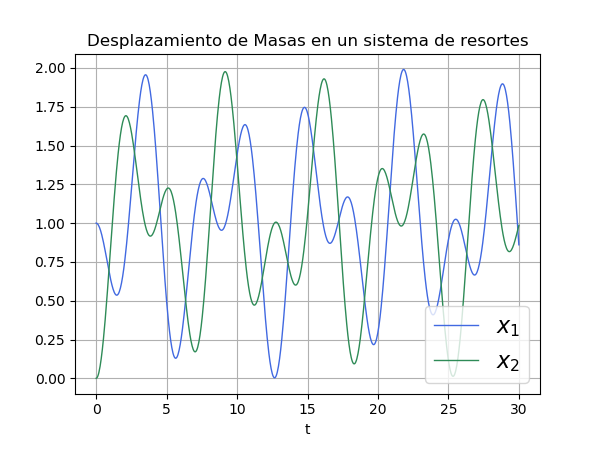
\includegraphics[width=0.65\textwidth]{imagen.png}
\end{figure}
\end{document}
